% ==========
% ANNEXES
% ==========

\renewcommand{\appendixtocname}{Annexes}
\renewcommand{\appendixpagename}{Annexes}

\begin{appendices}

On liste ici de nombreux résultats d'analyse fonctionnelle utilisés dans le rapport, et plus précisément des résultats sur la théorie des semi-groupes, la théorie des opérateurs compacts et la théorie spectrale issus de \cite{Brezis1987,Engel1991,Clement1987,Pazy1983,Webb1985}.

% ==============
% Annexe A
% ==============

% ------------------------------------------------------------
\section{Semi-groupes}\label{annexe_SG}
% ------------------------------------------------------------
Dans toute cette section, on considère un espace de Banach $X$.

\subsection{Semi-groupe uniformément continu d'opérateurs bornés}
Voir \cite[p.~1]{Pazy1983}.
\begin{definition}
    Soit $\big\{T(t)\big\}_{t \geq 0}$ une famille d'opérateurs bornés de $X$ dans $X$, parametrée par un réel positif $t$. On dit que la famille $\big\{T(t)\big\}_{t \geq 0}$ est un \textcolor{astral}{semi-groupe d'opérateurs bornés sur $X$} si 
    \begin{itemize}
        \item[$(i)$] $T(0)=I$,
        \item[$(ii)$] $T(t+s)=T(t)T(s)$ pour tout $t,s \in \bbR_+$ (propriété des semi-groupes). 
    \end{itemize}
\end{definition}

\begin{definition}
    Soit $\big\{T(t)\big\}_{t \geq 0}$ un semi-groupe d'opérateurs bornés. L'opérateur $A$ défini par 
    \begin{equation*}
        D(A) = \Big\{ x \in X \ \ | \ \ \lim_{h \to 0} \frac{T(h)x-x}{h} \ \text{ existe } \Big\}
    \end{equation*}
    et pour $x \in D(A)$
    \begin{equation*}
        Ax = \lim_{h \to 0} \frac{T(h)x-x}{h}
    \end{equation*}
    est le \textcolor{astral}{générateur infinitésimal du semi-groupe $\big\{T(t)\big\}_{t \geq 0}$}, et $D(A)$ est le domaine de définition de $A$.
\end{definition}

\begin{definition}
    Soit $\big\{T(t)\big\}_{t \geq 0}$ un semi-groupe d'opérateurs bornés. On dit que le semi-groupe est \textcolor{astral}{uniformément continu} si 
    \begin{equation*}
        \lim_{s \to t} \vertiii{T(s)-T(t)}=0
    \end{equation*}
\end{definition}

\begin{theorem}\label{thm_equiv_generateur_op_borne}
    Un opérateur $A$ est le générateur infinitésimal d'un semi-groupe uniformément continu si et seulement si $A$ est un opérateur borné.
\end{theorem}

\begin{proof}
    $\boxed{\Longrightarrow}$ Soit $A$ un opérateur borné. On pose 
    \begin{equation*}
        T(t) = \ex^{tA} = \sum_{n=0}^{+\infty}\frac{(tA)^n}{n!}
    \end{equation*}
    La série converge normalement pour tout $t \geq 0$ et donc pour tout $t \geq 0$, $T(t)$ est bien défini. Il est clair que $\big\{T(t)\big\}_{t \geq 0}$. On a 
    \begin{equation*}
        \vertiii{T(t)-I} \leq t\vertiii{A}\ex^{t\vertiii{A}}
    \end{equation*}
    et 
    \begin{equation*}
        \vertiii{\frac{T(t)-I}{t}-A} \leq \vertiii{A}\max_{0\leq s \leq t}\vertiii{T(s)-I}
    \end{equation*}
    Donc $\big\{T(t)\big\}_{t \geq 0}$ est un semi-groupe uniformément continu dont le générateur infinitésimal est l'opérateur $A$. \\
    $\boxed{\Longleftarrow}$ Soit $\big\{T(t)\big\}_{t \geq 0}$ un semi-groupe uniformément continu. Soit $\rho >0$ assez petit pour que 
    \begin{equation*}
        \vertiii{I-\frac{1}{\rho}\int_0^\rho T(s)\d s} <1
    \end{equation*}
    Alors $\rho^{-1}\displaystyle{\int_0^\rho} T(s)\d s$ est inversible et $\displaystyle{\int_0^\rho} T(s)\d s$ aussi. On a 
    \begin{eqnarray*}
        \frac{1}{h}(T(h)-I)\int_0^\rho T(s)\d s &=& \frac{1}{h}\bigg(\int_0^\rho T(s+h)\d s - \int_0^\rho T(s)\d s\bigg)\\
        &=& \frac{1}{h} \bigg(\int_\rho^{\rho+h}T(s)\d s - \int_0^hT(s)\d s\bigg)
    \end{eqnarray*}
    donc 
    \begin{equation*}
        \frac{1}{h}(T(h)-I) = \bigg(\frac{1}{h}\int_\rho^{\rho+h}T(s)\d s - \frac{1}{h}\int_0^hT(s)\d s\bigg)\bigg(\int_0^{\rho}T(s)\d s\bigg)^{-1}
    \end{equation*}
    En passant à la limite quand $h$ tend vers $0$, on obtient la convergence en norme de $h^{-1}(T(h)-I)$ et l'expression du générateur infinitésimal de $\big\{T(t)\big\}_{t \geq 0}$.
\end{proof}

\subsection{Forte continuité des semi-groupes d'opérateurs bornés}
Voir \cite{Pazy1983} section $1.2$.
\begin{definition}
    Soit $\big\{T(t)\big\}_{t \geq 0}$ un semi-groupe d'opérateurs bornés. On dit que le semi-groupe $\big\{T(t)\big\}_{t \geq 0}$ est \textcolor{astral}{continu au sens fort} si 
    \begin{equation*}
        \forall x \in X, \ \lim_{t \to 0} T(t)x=x
    \end{equation*}
    On dit que le semi-groupe $\big\{T(t)\big\}_{t \geq 0}$ est un \textcolor{astral}{$\scrC^0$ semi-groupe}.
\end{definition}

\begin{theorem}\label{thm_estimation_SG}
    Soit $\big\{T(t)\big\}_{t \geq 0}$ un $\scrC^0$ semi-groupe. Alors il existe $\omega \geq 0$ et $M \geq 1$ tels que 
    \begin{equation*}
        \forall t \in \bbR_+, \ \vertiii{T(t)} \leq M\ex^{\omega t}
    \end{equation*}
\end{theorem}

\begin{proof}
    Supposons par l'absurde que $(\vertiii{T(t)})_{t \geq 0}$ n'est pas bornée. Alors il existe une suite $(t_n)_{n \in \bbN} \subset \bbR_+$ qui tend vers $0$ telle que 
    \begin{equation*}
        \forall n \in \bbN, \ \vertiii{T(t_n)} \geq n
    \end{equation*}
    Alors par le théorème de Banach-Steinhaus il existe $x \in X$ tel que $(T(t_n)x)_{n \in \bbN}$ ne tend pas vers $x$. Ce qui contredit l'hypothèse de semi-groupe continu au sens fort. Donc il existe $\eta >0$ et $M\geq 0$ tels que 
    \begin{equation*}
        \forall t \in \ ]0,\eta[, \ \vertiii{T(t)} \leq M
    \end{equation*}
    De plus, comme $\vertiii{T(0)}=1$, on a $M \geq 1$. Posons $\omega :=\eta^{-1}\ln{(M)}$. Soit $t \geq 0$. On peut écrire $t=n\eta+\delta$ avec $n \in \bbN$ et $0 \leq \delta \leq \eta$. Alors 
    \begin{equation*}
        \vertiii{T(t)} = \vertiii{T(\delta)T(\eta)^n} \leq M^{n+1} \leq MM^{t/\eta} = M\ex^{\omega t}
    \end{equation*}
\end{proof}

\begin{corollaire}
    Si $\big\{T(t)\big\}_{t \geq 0}$ est un $\scrC^0$ semi-groupe alors pour tout $x \in X$, l'application $t \mapsto T(t)x$ est continue.
\end{corollaire}

\begin{proof}
    Soient $t,h \geq 0$. On a 
    \begin{eqnarray*}
        \|T(t+h)x-T(t)x\| &=& \|T(t)T(h)x-T(t)x\| \\
        &=&\|T(t)(T(h)x-x)\| \\
        &\leq& \vertiii{T(t)}\|T(h)x-x\| \\
        &\leq& M\ex^{\omega t} \|T(h)x-x\| \underset{h \to 0}{\longrightarrow} 0
    \end{eqnarray*}
\end{proof}

\begin{theorem}\label{proprietes_SG}
    Soient $\big\{T(t)\big\}_{t \geq 0}$ un $\scrC^0$ semi-groupe et $A$ son générateur infinitésimal. Alors 
    \begin{enumerate}
        \item Pour tout $x \in X$, 
        \begin{equation*}
            \lim_{h \to 0} \frac{1}{h}\int_t^{t+h}T(s)x\d s = T(t)x
        \end{equation*}
        \item Pour tout $x \in X$, $\displaystyle{\int_0^t}T(s)x\d s \in D(A)$ et 
        \begin{equation*}
            A\bigg(\int_0^t T(s)x\d s\bigg) = T(t)x-x
        \end{equation*}
        \item Pour tout $x \in D(A)$, $T(t)x \in D(A)$ et 
        \begin{equation*}
            \frac{\d}{\d t}T(t)x = AT(t)x=T(t)Ax
        \end{equation*}
        \item Pour tout $x \in D(A)$
        \begin{equation*}
            T(t)x-T(s)x = \int_s^tT(\tau)Ax\d \tau = \int_s^t AT(\tau)x\d \tau
        \end{equation*}
    \end{enumerate}
\end{theorem}

\begin{proof}
    \begin{enumerate}
        \item Soit $x \in X$. On a 
        \begin{equation*}
            \frac{1}{h}\int_t^{t+h}T(s)x\d s -T(t)x = \frac{1}{h}\int_t^{t+h}\big(T(s)x-T(t)x\big)\d s
        \end{equation*}
        Soit $\varepsilon >0$. Par continuité de $t \mapsto T(t)x$, il existe $\eta >0$ tel que 
        \begin{equation*}
            |s-t| < \eta \Longrightarrow \|T(s)x-T(t)x\| < \varepsilon
        \end{equation*}
        Pour $h \in \ ]0,\eta [$, si $s \in [t,t+h]$ alors $|s-t| \leq h < \eta$ donc 
        \begin{eqnarray*}
            \bigg\|\frac{1}{h}\int_t^{t+h}\big(T(s)x-T(t)x\big)\d s \bigg\| \leq \frac{1}{h}\int_t^{t+h}\|T(s)x-T(t)x\|\d s < \frac{1}{h}\int_t^{t+h}\varepsilon \d s < \varepsilon
        \end{eqnarray*}
        \item Soient $x \in X$ et $h >0$.
        \begin{eqnarray*}
            \frac{T(h)-I}{h}\int_0^tT(s)x \d s&=& \frac{1}{h}\int_0^t\big(T(s+h)x-T(s)x\big)\d s \\
            &=& \frac{1}{h}\int_0^t T(s+h)x\d s - \frac{1}{h}\int_0^tT(s)x\d s \\
            &=& \frac{1}{h}\int_h^{t+h}T(s)x\d s - \frac{1}{h}\int_0^t T(s)x\d s \\
            &=& \frac{1}{h}\int_t^{t+h}T(s)x\d s - \frac{1}{h}\int_0^h T(s)x\d s
        \end{eqnarray*}
        En passant à la limite dans cette égalité et en utilisant le premier point, on obtient l'égalité.
        \item Soient $x \in D(A)$ et $h>0$.
        \begin{eqnarray*}
            \frac{T(h)-I}{h}T(t)x = T(t)\bigg(\frac{T(h)-I}{h}\bigg)h \underset{h \to 0}{\longrightarrow} AT(t)x
        \end{eqnarray*}
        Donc $T(t)x \in D(A)$ et $AT(t)x=T(t)Ax$. On a aussi montré que la dérivée à droite de $T(t)x$ est $T(t)Ax$. Il nous faut maintenant montrer que la dérivée à gauche est $T(t)Ax$. On a 
        \begin{eqnarray*}
            \lim_{h \to 0} \bigg(\frac{T(t)x-T(t-h)x}{h}-T(t)Ax\bigg) &=& \lim_{h \to 0} T(t-h)\bigg(\frac{T(h)x-x}{h}-Ax\bigg) \\
            &+& \lim_{h \to 0}\big(T(t-h)Ax-T(t)Ax\big)
        \end{eqnarray*}
        Le terme de droite tend vers $0$, en effet le premier terme tend vers $0$ car $x \in D(A)$ et $\vertiii{T(t-h)}$ est borné pour $0\leq h \leq t$ et le second terme tend vers $0$ par forte continuité du semi-groupe.
        \item Il suffit d'intégrer l'égalité du point $3$ entre $s$ et $t$.
    \end{enumerate}
\end{proof}

\begin{corollaire}\label{cor_domaine_dense_op_ferme}
    Si $A$ est le générateur infinitésimal d'un $\scrC^0$ semi-groupe $\big\{T(t)\big\}_{t \geq 0}$, alors $D(A)$ est dense dans $X$ et $A$ est fermé.
\end{corollaire}

\begin{proof}
    Soit $x \in X$. On pose pour tout $t>0$
    \begin{equation*}
        x_t = \frac{1}{t}\int_0^tT(s)x\d s
    \end{equation*}
    On a $x_t \in D(A)$ par le point $2$ du théorème précédente et par le point $1$ on a
    \begin{equation*}
        x_t \underset{t \to 0}{\longrightarrow} T(0)x=x
    \end{equation*}
    donc $\overline{D(A)}=X$. Soit $(x_n)_{n \in \bbN} \subset D(A)$ telle que $x_n \longrightarrow x$ et $Ax_n \longrightarrow y$ où $x,y \in X$. On veut montrer que $Ax=y$ et $x \in D(A)$. Par le point $4$ on a 
    \begin{equation*}
        T(t)x_n-x_n=\int_0^tT(s)Ax_n\d s
    \end{equation*}
    Par continuité de $t \mapsto T(t)z$, on a en passant à la limite et par convergence dominée 
    \begin{equation*}
        T(t)x-x = \int_0^t T(s)y\d s
    \end{equation*}
    On divise par $t>0$ et on passe à la limite quand $t$ tend vers $0$, ce qui donne par le point $1$ du théorème précédent $x \in D(A)$ et $Ax=y$.
\end{proof}

\subsection{Le théorème de Hille-Yosida}
Voir \cite{Pazy1983} section $1.3$.
\begin{definition}
    Soit $\big\{T(t)\big\}_{t \geq 0}$ un $\scrC^0$ semi-groupe. Par le théorème \ref{thm_estimation_SG}, on a 
    \begin{equation*}
        \forall t \in \bbR_+, \ \vertiii{T(t)} \leq M\ex^{\omega t}
    \end{equation*}
    \begin{itemize}
        \item Si $\omega = 0$, on dit que le semi-groupe $\big\{T(t)\big\}_{t \geq 0}$ est \textcolor{astral}{uniformément borné}.
        \item Si $\omega = 0$ et $M=1$, on dit que le semi-groupe $\big\{T(t)\big\}_{t \geq 0}$ est un \textcolor{astral}{$\scrC^0$ semi-groupe de contractions}.
    \end{itemize}
\end{definition}

\begin{definition}
    Soit $A$ un opérateur de $X$ dans $X$. 
    \begin{itemize}
        \item On appelle \textcolor{astral}{ensemble resolvant de $A$}, l'ensemble $\rho(A)$ des $\lambda \in \bbC$ tels que $\lambda I-A$ est inversible, \textit{i.e.} $(\lambda I-A)^{-1}$ est un opérateur borné de $X$.
        \item La famille $R(\lambda : A):=(\lambda I-A)^{-1}$, où $\lambda \in \rho(A)$, est appelée la \textcolor{astral}{résolvante de $A$}.
    \end{itemize}
\end{definition}

\begin{theorem}[Hille-Yosida]\label{thm_HY}
    Un opérateur $A$ est le générateur infinitésimal d'un $\scrC^0$ semi-groupe de contractions $\big\{T(t)\big\}_{t \geq 0}$ si et seulement si 
    \begin{itemize}
        \item[$(i)$] $A$ est fermé et $\overline{D(A)}=X$,
        \item[$(ii)$] $\bbR_+ \subset \rho(A)$ et on a 
        \begin{equation*}
            \forall \lambda >0, \ \vertiii{R(\lambda : A)} \leq \frac{1}{\lambda}
        \end{equation*} 
    \end{itemize}
\end{theorem}

\begin{proof}
    $\boxed{\Longrightarrow}$ On sait déjà par le corollaire \ref{cor_domaine_dense_op_ferme} que $A$ est fermé et $D(A)$ est dense dans $X$. On pose pour $\lambda >0$ et $x \in X$
    \begin{equation*}
        R(\lambda)x=\int_0^{+\infty}\ex^{-\lambda t}T(t)x\d t
    \end{equation*}
    Comme $t \mapsto T(t)x$ est continue et uniformément bornée, l'intégrale est bien définie et $R(\lambda)$ est un opérateur qui vérifie 
    \begin{eqnarray*}
        \|R(\lambda)x\| \leq \int_0^{+\infty}\ex^{-\lambda t}\|T(t)x\|\d t \leq \|x\| \int_0^{+\infty}\ex^{-\lambda t}\d t=\frac{1}{\lambda}\|x\|
    \end{eqnarray*}
    donc $\vertiii{R(\lambda)} \leq 1/\lambda$. Montrons que $(\lambda I-A)R(\lambda)=I$. Soit $x \in X$.
    \begin{eqnarray*}
        (\lambda I-A)R(\lambda)x &=& \lambda R(\lambda)x-AR(\lambda)x \\
        &=& \lambda R(\lambda)x - \lim_{h \to 0}\frac{T(h)-I}{h}R(\lambda)x \\
        &=& \lambda R(\lambda)x-\lim_{h \to 0}\frac{1}{h}\bigg(\int_0^{+\infty}\ex^{-\lambda t}\big(T(t+h)-T(t)\big)x\d t\bigg) \\
        &=& \lambda R(\lambda)x-\lim_{h \to 0}\frac{1}{h}\bigg(\int_0^{+\infty}\ex^{-\lambda t}T(t+h)x-\int_0^{+\infty}\ex^{-\lambda t}T(t)x\d t\bigg) \\
        &=& \lambda R(\lambda)x-\lim_{h \to 0}\frac{1}{h}\bigg(\int_h^{+\infty}\ex^{-\lambda (t-h)}T(t)x\d t-\int_0^{+\infty}\ex^{-\lambda t}T(t)x\d t\bigg) \\
        &=& \lambda R(\lambda)x-\lim_{h \to 0}\bigg(\frac{\ex^{\lambda t}-1}{h}\int_0^{+\infty}\ex^{-\lambda t}T(t)x\d t-\frac{\ex^{\lambda h}}{h}\int_0^{h}\ex^{-\lambda t}T(t)x\d t\bigg) \\
        &=& \lim_{h \to 0} \frac{\ex^{\lambda h}}{h} \int_0^h\ex^{-\lambda t}T(t)x\d t = x
    \end{eqnarray*}
    on a aussi montré que $R(\lambda)x \in D(A)$. Montrons que $R(\lambda)(\lambda I-A)=I$. Soit $x \in D(A)$.
    \begin{eqnarray*}
        R(\lambda)Ax &=& \int_0^{+\infty}\ex^{-\lambda t}T(t)Ax\d t \\
        &=& \int_0^{+\infty}\ex^{-\lambda t}AT(t)x\d t \\
        &=& \lim_{s \to +\infty} \int_0^s \ex^{-\lambda t}AT(t)x\d t \\
        &=& \lim_{s \to +\infty} A\bigg(\int_0^s \ex^{-\lambda t}T(t)x\d t\bigg) \\
        \text{par fermeture } &=& A \int_0^{+\infty}\ex^{-\lambda t}T(t)x\d t = AR(\lambda)x
    \end{eqnarray*}
    donc $R(\lambda)x \in D(A)$ et 
    \begin{eqnarray*}
        R(\lambda)(\lambda I-A)x &=& \lambda R(\lambda)x-R(\lambda)Ax \\
        &=& \lambda R(\lambda)x-AR(\lambda)x \\
        &=& (\lambda I -A)R(\lambda)x
    \end{eqnarray*}
    Donc $R(\lambda)$ est l'inverse de $\lambda I-A$ et existe pour tout $\lambda \in \bbR_+^*$ et est borné par $1/\lambda$.
    \\
    $\boxed{\Longleftarrow}$ Pour montrer ce sens, on a besoin de quelques lemmes.

    \begin{lemme}\label{lemme1_HY}
        Soit $A$ satisfaisant $(i)$ et $(ii)$ et soit $R(\lambda : A)=(\lambda I - A)^{-1}$. Alors pour tout $x \in X$
        \begin{equation*}
            \lim_{\lambda \to +\infty} \lambda R(\lambda : A)x=x
        \end{equation*}
    \end{lemme}

    \begin{proof}
        Soit $x \in D(A)$.
        \begin{eqnarray*}
            \|\lambda R(\lambda:A)x-x\| = \|AR(\lambda: A)x\| = 
            \|R(\lambda:A)Ax\| \leq \frac{1}{\lambda}\|Ax\| \underset{\lambda \to +\infty}{\longrightarrow} 0
        \end{eqnarray*}
        Par hypothèse, $\overline{D(A)}=X$ et $\vertiii{\lambda R(\lambda :A)} \leq 1$ donc pour tout $x \in X$,
        \begin{equation*}
            \lim_{\lambda \to +\infty} \lambda R(\lambda : A)x=x
        \end{equation*}
    \end{proof}

    \begin{definition}
        Pour tout $\lambda >0$, on définit \textcolor{astral}{l'approximation de Yosida de $A$} par 
        \begin{equation*}
            A_{\lambda} = \lambda AR(\lambda : A)=\lambda^2R(\lambda : A)-\lambda I
        \end{equation*}
    \end{definition}

    \begin{lemme}\label{lemme2_HY}
        Soit $A$ satisfaisant $(i)$ et $(ii)$. Si $A_{\lambda}$ est l'approximation de Yosida de $A$ alors pour tout $x \in D(A)$
        \begin{equation*}
            \lim_{\lambda \to +\infty} A_\lambda x=Ax
        \end{equation*}
    \end{lemme}

    \begin{proof}
        Soit $x \in D(A)$. On a par le lemme \ref{lemme1_HY}
        \begin{equation*}
            \lim_{\lambda \to +\infty}A_{\lambda}x = \lim_{\lambda \to +\infty}\lambda AR(\lambda : A)x=Ax
        \end{equation*}
    \end{proof}

    \begin{lemme}\label{lemme3_HY}
        Soit $A$ satisfaisant $(i)$ et $(ii)$. Si $A_{\lambda}$ est l'approximation de Yosida de $A$ alors $A_{\lambda}$ est le générateur infinitésimal du semi-groupe uniformément continu de contractions $\big\{\ex^{tA_{\lambda}}\big\}_{t \geq 0}$. De plus, pour tout $x \in X$ et pour tout $\lambda,\mu >0$ on a 
        \begin{equation*}
            \|\ex^{tA_{\lambda}}x-\ex^{tA_{\mu}}x\| \leq t\|A_{\lambda}x-A_{\mu}x\|
        \end{equation*}
    \end{lemme}

    \begin{proof}
        On a 
        \begin{eqnarray*}
            \vertiii{A_{\lambda}} \leq \lambda^2\vertiii{R(\lambda:A)}+\lambda \leq 2\lambda
        \end{eqnarray*}
        donc $A_{\lambda}$ est un opérateur borné. Par le théorème \ref{thm_equiv_generateur_op_borne} $A_{\lambda}$ est le générateur infinitésimal du semi-groupe uniformément continu $\big\{\ex^{tA_{\lambda}}\big\}_{t \geq 0}$. On a ensuite 
        \begin{equation*}
            \vertiii{\ex^{tA_{\lambda}}} = \vertiii{\ex^{t\lambda^2R(\lambda:A)-t\lambda}} \leq \ex^{-t\lambda}\ex^{t\lambda^2\vertiii{R(\lambda:A)}} \leq \ex^{-t\lambda}\ex^{t\lambda}=1
        \end{equation*}
        donc $\big\{\ex^{tA_{\lambda}}\big\}_{t \geq 0}$ est un semi-groupe de contractions. Par définition $\ex^{tA_{\lambda}}$, $\ex^{tA_{\mu}}$, $A_{\lambda}$ et $A_{\mu}$ commutent. Donc 
        \begin{eqnarray*}
            \|\ex^{tA_{\lambda}}x-\ex^{tA_{\mu}}x\| &=& \bigg\| \int_0^1 \frac{\d}{\d s}\big(\ex^{tsA_{\lambda}}\ex^{t(1-s)A_{\mu}}x\big)\d s\bigg\| \\
            &\leq& \int_0^1 t \|\ex^{tsA_{\lambda}}\ex^{t(1-s)}A_{\mu}(A_{\lambda}x-A_{\mu}x)\d s \\
            &\leq& t\|A_{\lambda}x-A_{\mu}x\|
        \end{eqnarray*}
    \end{proof}
    On peut à présent finir la preuve du théorème de Hille-Yosida. Soit $x \in D(A)$. Alors 
    \begin{eqnarray*}
        \|\ex^{tA_{\lambda}}x-\ex^{tA_{\mu}}x\| \overset{\text{lemme } \ref{lemme3_HY}}{\leq} t \|A_{\lambda}x-A_{\mu}x\| \leq t\|A_{\lambda}x-Ax\| + t \|Ax-A_{\mu}x\|
    \end{eqnarray*}
    Par le lemme \ref{lemme2_HY}, on sait que pour $x \in D(A)$ $A_{\lambda}x \underset{\lambda \to +\infty}{\longrightarrow} Ax$. Donc en passant à la limite quand $\lambda, \mu \to +\infty$ on montre que la suite $\big(\ex^{tA_{\lambda}}x\big)_{\lambda \in \bbR}$ est de Cauchy dans $X$ qui est un Banach, donc elle converge et elle converge uniformément sur les compacts. On note alors 
    \begin{equation*}
        \forall t \in \bbR_+, \ \forall x \in D(A), \ \lim_{\lambda \to +\infty} \ex^{tA_{\lambda}}x = T(t)x
    \end{equation*}
    Comme $D(A)$ est dense dans $X$ et $\vertiii{\ex^{tA_{\lambda}}} \leq 1$, on a 
    \begin{equation*}
        \forall t \in \bbR_+, \ \forall x \in X, \ \lim_{\lambda \to +\infty}\ex^{tA_{\lambda}}x=T(t)x
    \end{equation*}
    et la convergence est encore uniforme sur les compacts. On vérifie aisément que $\big\{T(t)\big\}_{t \geq 0}$ est un semi-groupe de contractions. De plus, $t \mapsto T(t)x$ est continue comme limite uniforme de $t \mapsto \ex^{tA_{\lambda}}x$ qui est continue. Donc $\big\{T(t)\big\}_{t\geq 0}$ est un $\scrC^0$ semi-groupe de contractions. Vérifions que $A$ est le générateur infinitésimal de $\big\{T(t)\big\}_{t\geq 0}$. Soit $x \in D(A)$. On a 
    \begin{equation}\label{HY_eq1}
        T(t)x-x = \lim_{\lambda \to +\infty} (\ex^{tA_{\lambda}}x-x) = \lim_{\lambda \to +\infty} \int_0^t \ex^{sA_{\lambda}}A_{\lambda}x\d s = \int_0^tT(s)Ax\d s
    \end{equation}
    Soit $B$ le générateur infinitésimal de $\big\{T(t)\big\}_{t\geq0}$. On divise \eqref{HY_eq1} par $t>0$ et on passe à la limite quand $t$ tend vers $0$, on obtient 
    \begin{equation}\label{HY_eq2}
        Bx=Ax
    \end{equation}
    donc $x \in D(B)$. Par hypothèse, $1 \in \rho(A)$ et par le sens $\boxed{\Longrightarrow}$ appliqué à $B$ on a $1 \in \rho(B)$. D'où 
    \begin{equation*}
        (I-B)D(A) = D(A)-BD(A) \overset{\eqref{HY_eq2}}{=} D(A)-AD(A) = (I-A)D(A) = X
    \end{equation*}
    Le même argument donne 
    \begin{equation*}
        D(B) = (I-B)^{-1}X = D(A)
    \end{equation*}
    donc $A=B$.
\end{proof}

\begin{remark}\label{rq_SG}
    Soit $\big\{T(t)\big\}_{t \geq 0}$ un $\scrC^0$ semi-groupe tel que 
    \begin{equation*}
        \forall t \in \bbR_+, \ \vertiii{T(t)} \leq \ex^{\omega t}
    \end{equation*}
    On pose pour tout $t \in \bbR_+$, $S(t):=\ex^{-\omega t}T(t)$. Ainsi défini, $S(t)$ est un $\scrC^0$ semi-groupe de contractions. Si $A$ est le générateur infinitésimal de $T(t)$ alors $A-\omega I$ est le générateur infinitésimal de $(S(t))_{t \in \bbR_+}$. D'autre part, si $A$ est le générateur infinitésimal d'un $\scrC^0$ semi-groupe de contractions $(S(t))_{t \in \bbR_+}$, alors $A+\omega I$ est le générateur infinitésimal du $\scrC^0$ semi-groupe $\big\{T(t)\big\}_{t \geq 0}$ satisfaisant $\vertiii{T(t)} \leq \ex^{\omega t}$. De plus, pour tout $t \in \bbR_+$, $T(t) = \ex^{\omega t}S(t)$.
    \\
    On peut donc caractériser les générateurs infinitésimaux des $\scrC^0$ semi-groupes $\big\{T(t)\big\}_{t \geq 0}$ satisfaisant pour tout $t \in \bbR_+$, $\vertiii{T(t)} \leq \ex^{\omega t}$.
\end{remark}

\begin{corollaire}\label{cor_HY}
    Un opérateur $A$ est le générateur infinitésimal d'un $\scrC^0$ semi-groupe $\big\{T(t)\big\}_{t \geq 0}$ satisfaisant pour tout $t \in \bbR_+$, $\vertiii{T(t)} \leq \ex^{\omega t}$ si et seulement si 
    \begin{itemize}
        \item[$(i)$] $A$ est fermé et $\overline{D(A)}=X$,
        \item[$(ii)$] $\{\lambda \in \bbC \ \ | \ \ \Im(\lambda) = 0 \text{ et } \lambda > \omega \} \subset \rho(A)$ et on a pour $\lambda \in \{\lambda \in \bbC \ \ | \ \ \Im(\lambda) = 0 \text{ et } \lambda > \omega \}$
        \begin{equation}\label{eq_H-Y}
            \forall \lambda >0, \ \vertiii{R(\lambda:A)} \leq \frac{1}{\lambda-\omega}
        \end{equation} 
    \end{itemize}
\end{corollaire}

\begin{proof}
    Il suffit de combiner la remarque précédente au théorème de Hille-Yosida.
\end{proof}

\subsection{Opérateurs et semi-groupes compacts}
Voir \cite{Brezis1987} chapitre 6, \cite{Pazy1983} section $2.3$, \cite{Clement1987} annexe $3$ et \cite[p.~117]{Engel1991}.
\subsubsection{Opérateurs compacts et spectre d'opérateurs compacts}
Soient $E$ et $F$ deux espaces de Banach. On note $B_E$ la boule unité ouverte de $E$.
\begin{definition}
    On dit qu'un opérateur $T \in \scrL(E,F)$ est \textcolor{astral}{compact} si $T(\overline{B_E})$ est relativement compact pour la topologie forte. On désigne par $\scrK(E,F)$ l'ensemble des opérateurs compacts de $E$ dans $F$ et on pose $\scrK(E):=\scrK(E,E)$.
\end{definition}

\begin{proposition}\label{prop_op_compact_ferme}
    L'ensemble $\scrK(E,F)$ est un sous-espace vectoriel fermé de $\scrL(E,F)$.
\end{proposition}

\begin{proof}
    Il est clair que $\scrK(E,F)$ est un sous-espace vectoriel de $\scrL(E,F)$. Soit $(T_n)_{n \in \bbN} \subset \scrK(E,F)$ tel que $T_n \underset{n \to +\infty}{\longrightarrow} T \in \scrL(E,F)$. Montrons que $T \in \scrK(E,F)$. Comme $F$ est complet il suffit de vérifier que pour tout $\varepsilon >0$, $T(\overline{B_E})$ peut être recouvert par un nombre fini de boules $B(y_i,\varepsilon)$ dans $F$. On fixe $n$ tel que 
    \begin{equation*}
        \vertiii{T_n-T} < \frac{\varepsilon}{2}
    \end{equation*}
    Comme $T_n(\overline{B_E})$ est relativement compact, il existe un ensemble fini $I$ tel que 
    \begin{equation*}
        T_n(\overline{B_E}) \subset \bigcup_{i \in I}B_F\Big(y_i, \frac{\varepsilon}{2}\Big)
    \end{equation*}
    Soit $y \in T(\overline{B_E})$. Alors il existe $x \in \overline{B_E}$ tel que $Tx = y$. On a par hypothèse
    \begin{eqnarray*}
        \exists i \in I, \ T_nx \in B_F\Big(y_i,\frac{\varepsilon}{2}\Big) \ \ \ &\text{ et }& \|T_nx-Tx\|_F \leq \vertiii{T_n-T}\|x\|_E < \frac{\varepsilon}{2}
    \end{eqnarray*}
    D'où, par inégalité triangulaire 
    \begin{equation*}
        \|Tx-y_i\|_F \leq \|Tx-T_nx\|_F + \|T_nx-y_i\|_F < \frac{\varepsilon}{2}+\frac{\varepsilon}{2}=\varepsilon
    \end{equation*}
    On a montré que 
    \begin{equation*}
        \forall y \in T(\overline{B_E}), \ \exists i \in I, \ y \in B_F(y_i,\varepsilon)
    \end{equation*}
    donc
    \begin{equation*}
        T(\overline{B_E}) \subset \bigcup_{i\in I} B_F(y_i,\varepsilon)
    \end{equation*}
\end{proof}

\begin{proposition}\label{prop_produit_compact_borne}
    Soient $E$, $F$ et $G$ trois espaces de Banach. Si $T \in \scrL(E,F)$ et $S \in \scrK(F,G)$ (resp. $T \in \scrK(E,F)$ et $S \in \scrL(F,G)$) alors $S \circ T \in \scrK(E,G)$.
\end{proposition}

\begin{proof}
    \begin{itemize}
        \item Comme $T \in \scrL(E,F)$, $T(\overline{B_E}) \subset \overline{B_F(0,\vertiii{T})}$. Comme $S \in \scrK(F,G)$, $S$ envoie les bornés sur les ensembles relativement compact, donc $S\big(\overline{B_F(0,\vertiii{T})}\big)$ est relativement compact et
        \begin{equation*}
            S\big(T(\overline{B_E})\big) \subset S\big(\overline{B_F(0,\vertiii{T})}\big)
        \end{equation*}
        Donc $S \circ T \in \scrK(E,G)$.
        \item Comme $T \in \scrK(E,F)$, $T(\overline{B_E})$ est relativement compact dans $F$, donc $\overline{T(\overline{B_E})}$ est compact dans $F$. Comme $S \in \scrL(E,F)$, $S\big( \overline{T(\overline{B_E})}\big)$ est compact dans $G$. Et on a 
        \begin{equation*}
            S\big(T(\overline{B_E})\big) \subset S\big( \overline{T(\overline{B_E})}\big)
        \end{equation*}
        donc $S\big(T(\overline{B_E})\big)$ est relativement compact, donc $S \circ T \in \scrK(E,G)$.
    \end{itemize}
\end{proof}

\begin{definition}
    Soit $T \in \scrL(E)$. Le \textcolor{astral}{spectre de $T$} est 
    \begin{equation*}
        \sigma(T) := \bbC \setminus \rho(T)
    \end{equation*}
    On dit que $\lambda$ est une \textcolor{astral}{valeur propre de $T$} si 
    \begin{equation*}
        \ker (\lambda I - T) \neq \{0\}
    \end{equation*}
    et on note $\mathrm{VP}(T)$ l'ensemble des valeurs propres de $T$. Enfin, $\ker(\lambda I-T)$ est \textcolor{astral}{l'espace propre} associé à $\lambda$.
\end{definition}

\begin{definition}
    Soit $T \in \scrL(E)$. Le \textcolor{astral}{spectre essentiel de $T$} est l'ensemble des $\lambda \in \bbC$ tels que une des trois conditions est vérifiée 
    \begin{enumerate}
        \item $\lambda$ est un point limite de $\sigma(T)$,
        \item $\im(\lambda I - T)$ n'est pas fermé,
        \item $\displaystyle{\bigcup_{k=1}^{+\infty}} \im\big((\lambda I - T)^k\big)$ est de dimension infinie.
    \end{enumerate}
    On note $\sigma_{\text{ess}}(T)$ le spectre essentiel de $T$.
\end{definition}

\begin{theorem}[Riesz-Schauder]\label{thm_Riesz_Schauder}
    Soit $T \in \scrK(E)$ avec $\dim E = +\infty$. Alors on a 
    \begin{enumerate}
        \item $0 \in \sigma(T)$,
        \item $\sigma(T) \setminus \{0\} = \mathrm{VP}(T) \setminus \{0\}$,
        \item l'une des situations suivantes 
        \begin{itemize}
            \item ou bien $\sigma(T)=\{0\}$,
            \item ou bien $\sigma(T) \setminus \{0\}$ est fini,
            \item ou bien $\sigma(T)\setminus \{0\}$ est une suite de points isolés qui tend vers $0$.
        \end{itemize}
    \end{enumerate}
\end{theorem}

\begin{proof}
    Voir Théorème $6.8$ page $95$ de \cite{Brezis1987}.
\end{proof}

\subsubsection{Semi-groupes compacts}
\begin{definition}
    Un $\scrC^0$ semi-groupe $\big\{T(t)\big\}_{t \geq 0}$ est \textcolor{astral}{éventuellement compact} si pour tout $t>t_0$, $T(t)$ est un opérateur compact. Et on dit que $\big\{T(t)\big\}_{t \geq 0}$ est \textcolor{astral}{compact} si pour tout $t>0$, $T(t)$ est un opérateur compact.
\end{definition}

\begin{theorem}\label{thm_SG_compact_res}
    Soient $\big\{T(t)\big\}_{t \geq 0}$ un $\scrC^0$ semi-groupe et $A$ son générateur infinitésimal. Si $R(\lambda : A)$ est compact pour $\lambda \in \rho(A)$ et $t \mapsto T(t)$ est continue pour la topologie des opérateurs pour tout $t>t_0$, alors $T(t)$ est compact pour tout $t>t_0$. Autrement dit, $\big\{T(t)\big\}_{t \geq 0}$ est éventuellement compact.
\end{theorem}

\begin{proof}
    Soit $t>t_0$. On a pour tout $\lambda$ tel que $\Re \lambda > \omega$
    \begin{equation*}
        \lambda R(\lambda : A)T(t)-T(t) = \lambda \int_0^{+\infty}\ex^{-\lambda s}\big(T(t+s)-T(t)\big)\d s
    \end{equation*}
    Si on suppose $\lambda \in \bbR$ vérifiant $\lambda >\omega$, alors on a pour tout $\delta >0$
    \begin{eqnarray*}
        \vertiii{\lambda R(\lambda : A)T(t)-T(t)} &\leq& \int_0^{\delta} \lambda \ex^{-\lambda s}\vertiii{T(t+s)-T(t)}\d s+\int_{\delta}^{+\infty}\lambda \ex^{-\lambda s}\vertiii{T(t+s)-T(t)}\d s \\
        &\leq& \sup_{0\leq s \leq \delta} \vertiii{T(t+s)-T(t)} (1-\ex^{-\lambda \delta}) + M\ex^{\omega t}\int_{\delta}^{+\infty}\lambda \ex^{-s(\lambda-\omega)}\d s \\
        &+& M\ex^{\omega t}\int_{\delta}^{+\infty}\lambda \ex^{-\lambda s}\d s \\
        &\leq& \sup_{0\leq s \leq \delta} \vertiii{T(t+s)-T(t)}+M\ex^{\omega t}\lambda \frac{\ex^{-\delta \lambda}\ex^{\omega \delta}}{\lambda-\omega} + M\ex^{\omega t}\ex^{-\delta \lambda} \\
        &=& \sup_{0\leq s \leq \delta} \vertiii{T(t+s)-T(t)}+M \ex^{\omega t}\ex^{-\delta \lambda}\Big(\frac{\lambda}{\lambda-\omega}\ex^{\omega \delta}+1\Big)
    \end{eqnarray*}
    d'où 
    \begin{equation*}
        \forall \delta >0, \ \limsup_{\lambda \to +\infty} \vertiii{\lambda R(\lambda : A)T(t)-T(t)} \leq \sup_{0\leq s \leq \delta} \vertiii{T(t+s)-T(t)}
    \end{equation*}
    Comme $\delta$ est quelconque et $t \mapsto T(t)$ est continue pour $t>t_0$ en norme d'opérateurs, on a 
    \begin{equation*}
        \sup_{0\leq s \leq \delta} \vertiii{T(t+s)-T(t)} \underset{\delta \to 0}{\longrightarrow} 0
    \end{equation*}
    comme le membre de gauche de l'inégalité précédente ne dépend pas de $\delta$, on obtient
    \begin{equation*}
        \lim_{\lambda \to +\infty} \vertiii{\lambda R(\lambda : A)T(t)-T(t)} =0
    \end{equation*}
    Autrement dit, on a 
    \begin{equation*}
        \lim_{\lambda \to +\infty} \lambda R(\lambda : A)T(t)=T(t)
    \end{equation*}
    en norme d'opérateurs. Comme $\lambda R(\lambda : A)$ est compact et $T(t)$ est borné, on a par la proposition \ref{prop_produit_compact_borne} que $\lambda R(\lambda : A)T(t)$ est compact et par la proposition \ref{prop_op_compact_ferme} on sait que $\scrK(X)$ est fermé donc $T(t)$ est compact.
\end{proof}

\begin{proposition}\label{prop_injec_compacte}
    Soit $A$ un opérateur sur $X$ défini sur $D(A)$ tel que $\rho(A) \neq \emptyset$. Alors les assertions suivantes sont équivalentes
    \begin{itemize}
        \item[$(i)$] La résolvante de $A$ est compacte.
        \item[$(ii)$] L'injection $\big(D(A),\|\cdot\|_A\big) \hookrightarrow X$ est compacte, où $\|\cdot\|_A:=\|\cdot\| + \|A\cdot\|$ est la norme du graphe.
    \end{itemize}
\end{proposition}

\begin{proof}
    Soit $\lambda \in \rho(A)$. On a le diagramme suivant 
    \begin{center}
    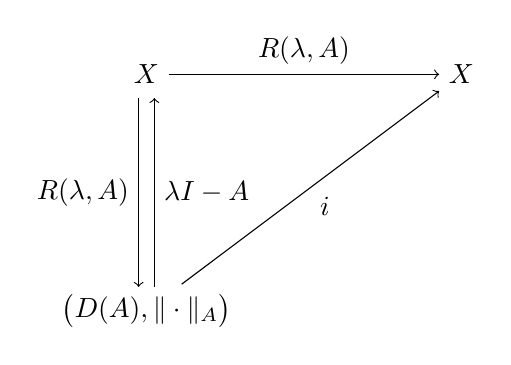
\begin{tikzpicture}[node distance=3cm, auto]

    % Noeuds
    \node (X1) at (0, 0)   {$X$};
    \node (X2) at (4, 0)   {$X$};
    \node (X3) at (0, -3)  {$\big(D(A),\|\cdot\|_A\big)$};

    % Flèche X -> X (en haut)
    \draw[->] (X1) -- (X2) node[midway, above] {$R(\lambda, A)$};

    % Flèche double X <-> X1 (à gauche)
    \draw[->] (-0.1,-0.3) -- (-0.1,-2.7) node[midway, left] {$R(\lambda, A)$};
    \draw[<-] (0.1,-0.3) -- (0.1,-2.7) node[midway, right] {$\lambda I-A$};

    % Flèche diagonale X1 -> X (en bas à droite)
    \draw[->] (X3) -- (X2) node[midway, below right] {$i$};

    \end{tikzpicture}
    \end{center}
    $\boxed{(i) \Longrightarrow (ii)}$ Le diagramme nous donne 
    \begin{equation*}
        i = R(\lambda : A)(\lambda I -A)
    \end{equation*}
    où on utilise $R(\lambda : A):X \rightarrow X$. Il nous suffit de montrer que $\lambda I - A : \big(D(A),\|\cdot\|_A\big) \rightarrow X$ est borné, alors $i$ sera compacte par la proposition \ref{prop_produit_compact_borne}. On a 
    \begin{equation*}
        \|(\lambda I - A)x\| \leq |\lambda| \|x\| + \|Ax\| \leq \max\{1,|\lambda|\}\|x\|_A
    \end{equation*}
    d'où la compacité de $i$.
    \\
    $\boxed{(ii) \Longrightarrow (i)}$ Le diagramme nous donne 
    \begin{equation*}
        R(\lambda : A) = i (\lambda I-A)^{-1}
    \end{equation*}
    où on utilise $R(\lambda : A) : X \rightarrow X$ et $(\lambda I-A)^{-1}: \big(D(A),\|\cdot\|_A\big) \rightarrow X$. Il nous suffit de montrer que $(\lambda I - A)^{-1} : X \rightarrow \big(D(A),\|\cdot\|_A\big)$ est borné, alors $R(\lambda : A):X \rightarrow X$ sera compacte par la proposition \ref{prop_produit_compact_borne}. On sait que $R(\lambda : A) : X \rightarrow X$ est borné, donc 
    \begin{eqnarray*}
        \|(\lambda I - A)^{-1}x\|_A &=& \|(\lambda I-A)^{-1}x\|+\|A(\lambda I - A)^{-1}x\| \\
        &\leq& \vertiii{R(\lambda : A)}\|x\| + \|\lambda(\lambda I - A)^{-1}x-\lambda(\lambda I-A)^{-1}x+A(\lambda I - A)^{-1}x\| \\
        &\leq& \vertiii{R(\lambda :A)}\|x\|+\|(\lambda I -A)(\lambda I - A)^{-1}x\| + |\lambda|\|(\lambda I -A)^{-1}x\| \\
        &\leq& \big(\vertiii{R(\lambda : A)}+|\lambda|\vertiii{R(\lambda :A)}+1\big)\|x\|
    \end{eqnarray*}
    d'où la compacité de $R(\lambda : A):X\rightarrow X$.
\end{proof}

\begin{definition}
    Soit $\Omega \subset X$ un ensemble borné. On définit la \textcolor{astral}{mesure de non-compacité de $\Omega$} par 
    \begin{equation*}
        \alpha(\Omega) := \inf\Big\{ d>0 \ |\ \exists \Omega_1,\dots,\Omega_n \subset X, \ \forall i \in \llbracket 1,n\rrbracket, \ \mathrm{diam}(\Omega_i) \leq d \text{ et } \Omega \subset \bigcup_{i=1}^n \Omega_i \Big\}
    \end{equation*}
\end{definition}

%\begin{proposition}
%    Soit $\Omega \subset X$ un ensemble borné.
%    \begin{enumerate}
%        \item $\alpha(\Omega)=0$ si et seulement si $\overline{\Omega}$ est compact.
%    \end{enumerate}
%\end{proposition}

%\begin{proof}
%
%\end{proof}

\begin{definition}
    Soit $T \in \scrL(X)$. On définit la \textcolor{astral}{mesure de non-compacité de $T$} par 
    \begin{equation*}
        |T|_{\alpha} := \inf\big\{ k>0 \ | \ \alpha(T\Omega) \leq k \alpha(\Omega) \text{ pour toute partie bornée } \Omega \subset X \big\}
    \end{equation*}
\end{definition}

%\begin{proposition}
%    Soit $T \in \scrL(X)$.
%    \begin{enumerate}
%        \item $|T|_{\alpha} \leq \|T\|$
%        \item $|T|_{\alpha} = 0$ si et seulement si $T \in \scrK(X)$.
%    \end{enumerate}
%\end{proposition}

%\begin{proof}
%    
%\end{proof}

\subsection{Semi-groupes positifs}
Voir \cite{Clement1987} chapitres $7$, $8$ et $9$.
\subsubsection{Quelques rappels - compléments}
\begin{definition}
    Un \textcolor{astral}{treillis vectoriel} est un espace vectoriel ordonné $X$ tel que $\sup(x,y)$ et $\inf(x,y)$ existent pour tout $x,y \in X$.
\end{definition}

\paragraph{Notations.} A chaque élément $x \in X$, on associe sa partie positive et sa partie négative 
\begin{eqnarray*}
    x_+ := \sup(x,0) \ \ \ &\text{ et }& \ \ \ x_-:=\sup(-x,0)
\end{eqnarray*}

\begin{definition}
    Soit $(X,\|\cdot\|)$ un espace de Banach ordonné. On dit que $X$ est un \textcolor{astral}{treillis de Banach} si $X$ est un treillis vectoriel et 
    \begin{equation*}
        \forall x,y \in X, \ |x| \leq |y| \Longrightarrow \|x\| \leq \|y\|
    \end{equation*}
    où $|x|:=\sup(x,-x)$.
\end{definition}

\begin{definition}
    Soit $(X,\|\cdot\|)$ un espace de Banach. L'ensemble $X^+ \subset X$ est un \textcolor{astral}{cône positif} si $X^+$ est un ensemble non-vide, fermé vérifiant 
    \begin{enumerate}
        \item $X^++X^+ \subset X^+$,
        \item $\forall \lambda \geq 0, \lambda X^+ \subset X^+$,
        \item $X^+ \cap (-X^+) = \{0\}$.
    \end{enumerate} 
\end{definition}

\begin{definition}
    Soit $(X,\|\cdot\|)$ un espace de Banach ordonnée et soit un cône positif $X^+$. On dit que le cône positif $X^+$ est \textcolor{astral}{normal} s'il existe $\delta >0$ tel que 
    \begin{equation*}
        \forall x,y \in X, \ 0 \leq x \leq y \Longrightarrow \|x\| \leq \delta \|y\|
    \end{equation*}
\end{definition}

\begin{definition}
    Soit $(X,\|\cdot\|)$ un espace de Banach ordonnée et soit un cône positif $X^+$. On dit que le cône positif $X^+$ est \textcolor{astral}{générateur} si 
    \begin{equation*}
        X^+ - X^+ = X
    \end{equation*}
\end{definition}

\subsubsection{Semi-groupes positifs}
Soient $X$ un espace de Banach ordonné et $X^+$ un cône positif de $X$. Soit $\big\{T(t)\big\}_{t \geq 0}$ un $\scrC^0$ semi-groupe sur $X$ de générateur infinitésimal $A$.

\begin{definition}
    Le semi-groupe $\big\{T(t)\big\}_{t \geq 0}$ est \textcolor{astral}{positif} si pour tout $t \geq 0$ 
    \begin{equation*}
        T(t)X^+ \subset X^+
    \end{equation*}
\end{definition}

\begin{definition}
    On définit le \textcolor{astral}{type} de $\big\{T(t)\big\}_{t \geq 0}$ par 
    \begin{equation*}
        \omega_0 := \lim_{t \to +\infty}\frac{\ln(\vertiii{T(t)})}{t} = \inf_{t >0}\frac{\ln(\vertiii{T(t)})}{t}
    \end{equation*}
\end{definition}

\begin{definition}
    On définit le \textcolor{astral}{type essentiel} de $\big\{T(t)\big\}_{t \geq 0}$ par 
    \begin{equation*}
        \omega_{\text{ess}} := \lim_{t \to +\infty}\frac{\ln(|T(t)|_{\alpha})}{t} = \inf_{t >0}\frac{\ln(|T(t)|_\alpha)}{t}
    \end{equation*}
    où $|\cdot|_{\alpha}$ est la mesure de non-compacité.
\end{definition}

\begin{remark}
    On a $|T(t)|_{\alpha} \leq \vertiii{T(t)}$ pour tout $t \in \bbR_+$, donc 
    \begin{equation*}
        \omega_{\text{ess}} \leq \omega_0
    \end{equation*}
    Et, si le semi-groupe $\big\{T(t)\big\}_{t \geq 0}$ est éventuellement compact, alors $\omega_{\text{ess}}=-\infty$.
\end{remark}

\begin{definition}
    On définit la \textcolor{astral}{borne spectrale de $A$} par 
    \begin{equation*}
        s(A):= \sup\{\Re (\lambda) \in \bbR \ \ | \ \ \lambda \in \sigma(A)\}
    \end{equation*}
    avec $s(A)=-\infty$ si le spectre de $A$ est vide.
\end{definition}

\begin{definition}
    On définit 
    \begin{equation*}
        s_1(A):=\sup\{ \Re(\lambda) \in \bbR \ | \ \lambda \in \sigma(A) \setminus \sigma_{\text{ess}}(A)\}
    \end{equation*}
\end{definition}

\begin{remark}
    On a toujours 
    \begin{equation*}
        s_1(A) \leq s(A) \leq \omega_0
    \end{equation*}
\end{remark}

%\begin{theorem}\label{thm_borne_spect_et_resolvante}
%    On suppose que le cône positif $X^+$ est générateur et normal. Alors $s(A) = \sup\{\lambda \in \bbR \ | \ \lambda \in \sigma(A)\}$ et 
%    \begin{equation*}
%        R(\mu : A)x = \int_0^{+\infty} \ex^{-\mu t}T(t)x\d t
%    \end{equation*}
%    pour tout $x \in X$ et pour tout $\mu \in \bbC$ tel que $\Re(\mu) > s(A)$.
%\end{theorem}

%\begin{proof}
%    
%\end{proof}

\begin{definition}
    Un élément $u \in X$ tel que $u \geq 0$ est un 
    \textcolor{astral}{point quasi-intérieur} si $\overline{X_u}=X$, où
    \begin{equation*}
        X_u := \big\{ x \in X \ | \ \exists \lambda >0, \ -\lambda u \leq x \leq \lambda u \big\}
    \end{equation*}
    est l'idéal principal engendré par $u$.
\end{definition}

\begin{proposition}\label{prop_pts_quasi_inter}
    Soit $u \in X$ tel que $u \geq 0$. Alors $u$ est un point quasi-intérieur si et seulement si pour tout $\phi \in X'$ tel que $\phi >0$ on a $\langle u,\phi \rangle >0$.
\end{proposition}

\begin{proof}
    Admise.
\end{proof}

\begin{definition}
    Soit $J$ un idéal fermé de $X$. On dit que $J$ est 
    \textcolor{astral}{$\big\{T(t)\big\}_{t \geq 0}$ invariant} si pour tout $t \geq 0$ on a 
    \begin{equation*}
        T(t)J \subset J
    \end{equation*}
\end{definition}

\begin{definition}
    On dit que le semi-groupe $\big\{T(t)\big\}_{t \geq 0}$ est \textcolor{astral}{irréductible} si $\{0\}$ et $X$ sont les seuls idéaux fermés $\big\{T(t)\big\}_{t \geq 0}$ invariant.
\end{definition}

\begin{definition}\label{def_fort_irreductible}
    On dit que le semi-groupe $\big\{T(t)\big\}_{t \geq 0}$ est fortement irréductible si pour tout $t > 0$ et pour tout $u \in X$ tel que $u>0$, $T(t)u$ est un point quasi-intérieur.
\end{definition}

\begin{remark}
    Toutes ces définitions sont initialement valable pour des opérateurs quelconques. Ici on fait le choix de les énoncés dans le cadre des semi-groupes directement.
\end{remark}

\begin{proposition}\label{SG_irréductible}
    Soit $\big\{T(t)\big\}_{t \geq 0}$ un $\scrC^0$ semi-groupe de générateur infinitésimal $A$ sur un treillis de Banach $X$. Les assertions suivantes sont équivalentes
    \begin{itemize}
        \item[$(i)$] $\big\{T(t)\big\}_{t \geq 0}$ est irréductible.
        \item[$(ii)$] Pour tout $x \in X$ tel que $x>0$ et pour tout $\phi \in X'$ tel que $\phi>0$, il existe $t \geq 0$ tel que $\langle T(t)x,\phi\rangle >0$.
        \item[$(iii)$] $R(\lambda : A)$ est fortement irréductible pour tout $\lambda > s(A)$.
        \item[$(iv)$] $R(\lambda : A)$ est irréductible pour tout $\lambda >s(A)$.   
    \end{itemize}
\end{proposition}

\begin{proof}
    Voir Proposition $7.6$ page $165$ de \cite{Clement1987}.
\end{proof}

\subsubsection{Théorie de Perron-Frobenius pour les semi-groupes positifs}
Soient $X$ un espace de Banach ordonné et $X^+$ un cône positif de $X$. Soit $\big\{T(t)\big\}_{t \geq 0}$ un $\scrC^0$ semi-groupe sur $X$ de générateur infinitésimal $A$.

\begin{definition}
    On définit le \textcolor{astral}{rayon spectral} de $T(t)$ par 
    \begin{equation*}
        r(T(t)) := \ex^{\omega_0t}
    \end{equation*}
\end{definition}

\begin{definition}
    On définit le \textcolor{astral}{rayon spectral essentiel} de $T(t)$ par 
    \begin{equation*}
        r_{\text{ess}}(T(t)) := \ex^{\omega_{\text{ess}}t}
    \end{equation*}
\end{definition}

\begin{proposition}\label{prop_lien_type_borne_spectrale}
    On a 
    \begin{enumerate}
        \item $\sup\{\Re(\lambda) \in \bbR \ | \ \lambda \in \sigma_{\text{ess}}(A)\} \leq \omega_{\text{ess}}$
        \item $\omega_0 = \max\{s(A),\omega_{\text{ess}}\}=\max\{s_1(A), \omega_{\text{ess}}\}$
    \end{enumerate}
\end{proposition}

\begin{proof}
    Voir Proposition $8.6$ page $201$ de \cite{Clement1987}.
\end{proof}

\begin{definition}
    On définit le \textcolor{astral}{spectre périphérique de $A$} par 
    \begin{equation*}
        \sigma_+(A) := \{\lambda \in \sigma(A) \ | \ \Re(\lambda)=s(A)\}
    \end{equation*}
\end{definition}

\subsection{Comportement asymptotique}
\begin{theorem}\label{thm_asymptotique1}
    Soit $\big\{T(t)\big\}_{t \geq 0}$ un $\scrC^0$ semi-groupe positif tel que $\omega_{\text{ess}} < \omega_0$. Alors 
    \begin{enumerate}
        \item $\sigma_+(A)=\{s(A)\}$ et il existe $\varepsilon >0$ tel que 
        \begin{eqnarray*}
            \omega_{\text{ess}} \leq s(A)-\varepsilon \ \ \ &\text{ et }& \ \ \ \forall \lambda \in \sigma(A) \setminus \{s(A)\}, \ \Re(\lambda) \leq s(A)- \varepsilon
        \end{eqnarray*}
        \item De plus, si $\big\{T(t)\big\}_{t \geq 0}$ est irréductible alors $s(A)$ est un pôle d'ordre $1$ de $R(\lambda :A)$ de multiplicité géométrique $1$.
    \end{enumerate}
\end{theorem}

\begin{proof}
    Voir Théorème $9.10$ page $223$ de \cite{Clement1987}.
\end{proof}

\begin{theorem}\label{thm_asymptotique2}
    Soit $\big\{T(t)\big\}_{t \geq 0}$ un $\scrC^0$ semi-groupe positif tel que $\omega_{\text{ess}} < \omega_0$. On note $p$ l'ordre du pôle $\lambda_0=s(A)$ de $R(\lambda : A)$ et on note $P$ la projection de $\im\big((\lambda_0I-A)^p\big)$ sur lui-même. Et soit $\varepsilon >0$ donné par le théorème \ref{thm_asymptotique1}. Alors 
    \begin{enumerate}
        \item Pour tout $\eta \in \ ]0,\varepsilon[$ il existe une constante $M_\eta\geq 1$ telle que 
        \begin{equation*}
            \|T(t)(I-P)\| \leq M_\eta \ex^{(\lambda_0-\eta)t}
        \end{equation*}
        \item Si $p=1$, alors pour tout $\eta \in \ ]0,\varepsilon[$ on a 
        \begin{equation*}
            \|e^{-\lambda_0t}T(t)-P\| \leq M_\eta \ex^{-\eta t}
        \end{equation*}
        \item Si $\big\{T(t)\big\}_{t \geq 0}$ est irréductible et on a $x_0 \in X^+$ et $x_0^* \in (X')^+$ tels que 
        \begin{equation*}
            \begin{array}{ccccc}
                Ax_0 = \lambda_0x_0 && A^*x_0^* = \lambda_0x_0^* && \langle x_0,x_0^*\rangle =1
            \end{array}
        \end{equation*}
        alors pour tout $\eta \in \ ]0,\varepsilon[$ et pour tout $x \in X$, on a 
        \begin{equation*}
            \|\ex^{-\lambda_0t}T(t)x - \langle x,x_0^*\rangle x_0\| \leq M_\eta \ex^{-\eta t}\|x\|
        \end{equation*}
    \end{enumerate}
\end{theorem}

\begin{proof}
    Voir Théorème $9.11$ page $224$ de \cite{Clement1987}.
\end{proof}

\subsection{Problème de Cauchy abstrait}
Voir \cite{Pazy1983} section $4.1$.
\\\\
Soit un opérateur $A$ défini sur $D(A) \subset X$. Soit $x \in X$, le problème de Cauchy abstrait pour $A$ avec la donnée initiale $x$ consiste à trouver une solution $u(t)$ au problème 
\begin{equation}\label{pbmCauchyabstrait}
    \left\{\begin{array}{l}
        \dfrac{\d}{\d t}u(t) = Au(t) \ \ \ \ \ t >0 \\
        \\
        u(0)=x
    \end{array}\right.
\end{equation}
Par solution, on entend une fonction $u:\bbR_+ \rightarrow X$ continue, dérivable, telle que $u(t) \in D(A)$ pour tout $t >0$ et satisfaisant \eqref{pbmCauchyabstrait}. Si $u(t) \in D(A)$ pour tout $t>0$ et $u$ est continue en $t=0$, alors \eqref{pbmCauchyabstrait} n'admet pas de solution pour $x \notin \overline{D(A)}$.

\begin{lemme}\label{lemme1}
    Soient $T>0$ et $u:[0,T] \rightarrow X$ une fonction continue. S'il existe $M\geq 0$ tel que
    \begin{equation*}
        \forall n \in \bbN, \ \bigg\|\int_0^T \ex^{ns}u(s)\d s\bigg\| \leq M
    \end{equation*}
    alors $u(t)=0$ pour tout $t \in [0,T]$.
\end{lemme}

\begin{proof}
    Voir Lemme $1.1$ page $100$ de \cite{Pazy1983}.
\end{proof}

\begin{theorem}\label{thm_res_sol}
    Soit $A$ un opérateur défini sur un domaine dense dans $X$. Si $R(\lambda : A)$ existe pour tout réel $\lambda \geq \lambda_0$ et 
    \begin{equation*}
        \limsup_{\lambda \to +\infty} \frac{\ln\vertiii{R(\lambda:A)}}{\lambda} \leq 0
    \end{equation*}
    alors le problème \eqref{pbmCauchyabstrait} admet au plus une solution pour tout $x \in X$.
\end{theorem}

\begin{proof}
    Supposons que le problème \eqref{pbmCauchyabstrait} admette deux solutions $u_1(t)$ et $u_2(t)$. Alors pour tout $t \geq 0$, $u(t):=u_1(t)-u_2(t)$ est solution du problème 
    \begin{equation}\label{pbmCauchyabstrait_donnee_initiale_nulle}
        \left\{\begin{array}{l}
            \dfrac{\d}{\d t}u(t) = Au(t) \ \ \ \ \ t >0 \\
            \\
            u(0)=0
        \end{array}\right.
    \end{equation}
    Montrons que $u(t) = 0$ pour tout $t \geq 0$. On considère la fonction $t \mapsto R(\lambda : A)u(t)$ pour $\lambda \geq \lambda_0$. Comme $u$ est solution de \eqref{pbmCauchyabstrait_donnee_initiale_nulle} on a 
    \begin{eqnarray*}
        \frac{\d}{\d t}R(\lambda : A)u(t) &=& R(\lambda : A)Au(t) \\
        &=& R(\lambda :A)Au(t)-\lambda R(\lambda : A)u(t) + \lambda R(\lambda : A)u(t) \\
        &=& \lambda R(\lambda : A)u(t)-(\lambda I-A)R(\lambda : A)u(t) \\
        &=& \lambda R(\lambda : A)u(t)-u(t)
    \end{eqnarray*}
    La solution de cette équation est donnée par 
    \begin{equation*}
        R(\lambda : A)u(t) = \ex^{\lambda t}R(\lambda : A)u(0)-\int_0^t\ex^{\lambda(t-\tau)}u(\tau)\d \tau = -\int_0^t\ex^{\lambda(t-\tau)}u(\tau)\d \tau 
    \end{equation*}
    Par hypothèse,
    \begin{equation*}
        \limsup_{\lambda \to +\infty} \frac{\ln\vertiii{R(\lambda:A)}}{\lambda} \leq 0
    \end{equation*}
    donc 
    \begin{equation*}
        \forall \sigma >0, \ \lim_{\lambda \to +\infty}\ex^{-\sigma \lambda}\vertiii{R(\lambda :A)}=0
    \end{equation*}
    On a 
    \begin{eqnarray*}
        \ex^{-\sigma \lambda}\int_0^t\ex^{\lambda(t-\tau)}u(\tau)\d \tau = \ex^{-\sigma \lambda}\int_0^{t-\sigma}\ex^{\lambda(t-\tau)}u(\tau)\d \tau + \ex^{-\sigma \lambda}\int_{t-\sigma}^t \ex^{\lambda(t-\tau)}u(\tau)\d \tau
    \end{eqnarray*}
    ce qui donne 
    \begin{equation*}
        \int_0^{t-\sigma}\ex^{\lambda(t-\sigma-\tau)}u(\tau)\d\tau = -\ex^{-\sigma \lambda}R(\lambda : A)u(t)-\int_{t-\sigma}^t \ex^{\lambda (t-\sigma-\tau)}u(\tau)\d\tau
    \end{equation*}
    en appliquant la norme à cette égalité on obtient 
    \begin{eqnarray*}
        \bigg\|\int_0^{t-\sigma}\ex^{\lambda(t-\sigma-\tau)}u(\tau)\d\tau\bigg\| &\leq& \ex^{-\sigma \lambda}\vertiii{R(\lambda:A)}\|u(t)\| + \bigg\|\int_{t-\sigma}^t \ex^{\lambda (t-\sigma-\tau)}u(\tau)\d\tau\bigg\| \\
        &\leq& \ex^{-\sigma \lambda}\vertiii{R(\lambda:A)}\|u(t)\| + \frac{1-\ex^{-\sigma \lambda}}{\lambda}\sup_{t-\sigma \leq \tau \leq t}\|u(\tau)\| 
    \end{eqnarray*}
    Dans cette dernière égalité, on a bien l'existence du $\sup$ car $u$ est continue et $[t-\sigma,t]$ est compact. Le terme $\|u(t)\|$ ne pose pas de problème car $t$ est fixé et la norme ne dépend pas de $\lambda$. On peut à présent passer à la limite quand $\lambda$ tend vers $+\infty$, on obtient
    \begin{equation*}
        \lim_{\lambda \to +\infty}\int_0^{t-\sigma}\ex^{\lambda(t-\sigma-\tau)}u(\tau)\d\tau=0
    \end{equation*}
    Par le lemme \ref{lemme1}, $u(\tau)=0$ pour tout $\tau \in [0,t-\sigma]$. Comme $t$ et $\sigma$ sont quelconques, on a bien $u(t)=0$ pour tout $t \geq 0$. Finalement, $u_1(t)=u_2(t)$ pour tout $t \geq 0$.
\end{proof}

\subsection{Problème d'évolution non-linéaire}
Voir \cite{Pazy1983} section $3.1$, section $6.1$ et \cite[p.~199, p.~202, p.~206]{Webb1985}.
\\\\
Dans cette section, nous allons étudier le problème semi-linéaire
\begin{equation}\label{pbmCauchy_semilineaire}
    \left\{\begin{array}{l}
        \dfrac{\d}{\d t}u(t) +Au(t)=f\big(t,u(t)\big) \ \ \ \ \ t >t_0 \\
        \\
        u(t_0) = u_0
    \end{array}\right.
\end{equation}
où $-A$ est le générateur infinitésimal d'un $\scrC^0$ semi-groupe $\big\{T(t)\big\}_{t \geq 0}$ sur un espace de Banach $X$ et $f:[t_0,T] \times X \rightarrow X$ est un fonction continue en $t$ et satisfaisant une condition de Lipschitz en $u$.

\subsubsection{Existence et unicité}
\begin{definition}
    Une solution continue $u$ de l'équation intégrale
    \begin{equation*}
        u(t) = T(t-t_0)u_0 + \int_{t_0}^t T(t-s)f\big(s,u(s)\big)\d s
    \end{equation*}
    est appelée \textcolor{astral}{solution mild} du problème \eqref{pbmCauchy_semilineaire}.
\end{definition}

\begin{theorem}
    Soit $f:[t_0,T] \times X \rightarrow X$ continue en $t$ sur $[t_0,T]$ et uniformément Lipschitz de constante $L$ sur $X$. Si $-A$ est le générateur infinitésimal d'un $\scrC^0$ semi-groupe $\big\{T(t)\big\}_{t \geq 0}$ alors pour toute condition initiale $u_0 \in X$, le problème \eqref{pbmCauchy_semilineaire} admet une unique solution mild $u \in \scrC^0\big([t_0,T],X\big)$. De plus, l'application $u_0 \mapsto u$ est Lipschitzienne de $X$ dans $\scrC^0\big([t_0,T],X\big)$.
\end{theorem}

\begin{remark}
    C'est une généralisation du théorème de Cauchy-Lipschitz local.
\end{remark}

\begin{proof}
    Soit $u_0 \in X$. On considère l'application 
    \begin{equation*}
        F : \scrC^0\big([t_0,T],X\big) \rightarrow \scrC^0\big([t_0,T],X\big)
    \end{equation*}
    définie par 
    \begin{equation*}
        (Fu)(t) = T(t-t_0)u_0 + \int_{t_0}^t T(t-s)f\big(s,u(s)\big)\d s \ \ \ \ \ t_0 \leq t \leq T
    \end{equation*}
    On munit $\scrC^0\big([t_0,T],X\big)$ de la norme $\|\cdot\|_{\infty}$. On a donc 
    \begin{eqnarray*}
        \|(Fu)(t)-(Fv)(t)\| &=& \bigg\|\int_{t_0}^tT(t-s)\big(f\big(s,u(s)\big)-f\big(s,v(s)\big)\big)\d s\bigg\| \\
        &\leq& \int_{t_0}^t \vertiii{T(t-s)} \big\|f\big(s,u(s)\big)-f\big(s,v(s)\big)\big\|\d s \\
        &\leq& M \int_{t_0}^t \big\|f\big(s,u(s)\big)-f\big(s,v(s)\big)\big\|\d s \\
        &\leq& ML(t-t_0)\|u-v\|_{\infty}
    \end{eqnarray*}
    Comme $\big\{T(t)\big\}_{t \geq 0}$ est un $\scrC^0$ semi-groupe, il est localement borné, donc il existe $M>0$ tel que 
    \begin{equation*}
        \sup_{0 \leq t \leq T-t_0} \vertiii{T(t)} \leq M
    \end{equation*}
    Pour la dernière inégalité, on utilise l'hypothèse de Lipschitz sur $f$. On a ensuite 
    \begin{eqnarray*}
        \|(F^2u)(t)-(F^2v)(t)\| &\leq& ML \int_{t_0}^t \|(Fu)(s)-(Fv)(s)\| \d s\\
        &\leq& ML \int_{t_0}^t ML(s-t_0)\|u-v\|_{\infty}\d s \\
        &\leq& (ML)^2 \|u-v\|_{\infty}\frac{(t-t_0)^2}{2}
    \end{eqnarray*}
    Une récurrence immédiate donne pour tout $n \geq 1$
    \begin{equation*}
        \|(F^nu)(t)-(F^nv)(t)\| \leq \frac{\big(ML(t-t_0)\big)^n}{n!}\|u-v\|_{\infty} \leq \frac{(MLT)^n}{n!}\|u-v\|_{\infty}
    \end{equation*}
    Pour $n$ assez grand, on a $\dfrac{(MLT)^n}{n!}<1$, donc $F^n$ est contractante. Par le théorème du point fixe de Banach, l'application $F^n$ admet un unique point fixe $u \in \scrC^0\big([t_0,T],X\big)$. Comme 
    \begin{equation*}
        F^n(Fu)=F(F^nu) = Fu
    \end{equation*} 
    $Fu$ est aussi un point fixe de $F^n$, donc par unicité du point fixe, on a 
    \begin{equation*}
        Fu=u
    \end{equation*}
    donc $u$ est aussi un point fixe pour $F$.
    \\
    Montrons à présent l'unicité de la solution mild et la condition de Lipschitz sur l'application $u_0 \mapsto u$. Soit $v$ une solution mild de \eqref{pbmCauchyabstrait} sur $[t_0,T]$ de condition initiale $v_0 \in X$. Soit $t \in [t_0,T]$, on a 
    \begin{eqnarray*}
        \|u(t)-v(t)\| &\leq& \|T(t-t_0)u_0 -T(t-t_0)v_0\| + \int_{t_0}^t \big\|T(t-s)\big(f\big(s,u(s)\big)-f\big(s,v(s)\big)\big)\big\|\d s \\
        &\leq& M\|u_0-v_0\| +ML \int_{t_0}^t \|u(s)-v(s)\|\d s
    \end{eqnarray*}
    Par le lemme de Grönwall, on obtient 
    \begin{equation*}
        \forall t \in [t_0,T], \ \|u(t)-v(t)\| \leq M\ex^{ML(t-t_0)}\|u_0-v_0\| \leq M\ex^{ML(T-t_0)}\|u_0-v_0\|
    \end{equation*}
    donc 
    \begin{equation*}
        \|u-v\|_{\infty} \leq M\ex^{ML(T-t_0)}\|u_0-v_0\|
    \end{equation*}
    On obtient bien la condition de Lipschitz de l'application $u_0 \mapsto u$. Pour l'unicité, il suffit de prendre $v_0=u_0$, ainsi $u$ et $v$ sont solutions du même problème \ref{pbmCauchyabstrait} et on obtient 
    \begin{equation*}
        \|u-v\|_{\infty}=0 \iff \forall t \in [t_0,T], \ u(t)=v(t)
    \end{equation*}
    d'où l'unicité de la solution mild.
\end{proof}

\begin{definition}
    On dit que $f$ est \textcolor{astral}{localement Lipschitz en $u$ et uniformément continue en $t$ sur les compacts} si pour tout $t'\geq 0$ et pour toute constante $c\geq 0$ il existe une constante $L(c,t')$ telle que pour tout $u,v \in X$ vérifiant $\|u\|, \|v\| \leq c$ et pour tout $t \in [0,t']$ on ait 
    \begin{equation*}
        \|f(t,u)-f(t,v)\| \leq L(c,t')\|u-v\|
    \end{equation*}
\end{definition}

\begin{theorem}\label{CauchyLipschitz_explosiontempsfini}
    Soit $f:\bbR_+ \times X \rightarrow X$ continue sur $\bbR_+$ et localement Lipschitz en $u$ et uniformément continue en $t$ sur les compacts. Si $A$ est le générateur infinitésimal d'un $\scrC^0$ semi-groupe $\big\{T(t)\big\}_{t \geq 0}$ sur $X$, alors pour tout $u_0 \in X$ il existe $t_{\max} \leq +\infty$ tel que le problème \eqref{pbmCauchy_semilineaire} avec $t_0=0$ admet une unique solution mild $u$ sur $[0,t_{\max}[$. De plus, si $t_{\max}<+\infty$ alors 
    \begin{equation*}
        \lim_{t \to t_{\max}}\|u(t)\| = +\infty
    \end{equation*}
\end{theorem}

\begin{remark}
    C'est une généralisation du théorème de Cauchy-Lipschitz global et du théorème d'explosion en temps fini.
\end{remark}

\begin{proof}
    Voir Théorème $1.4$ page $185$ de \cite{Pazy1983}.
\end{proof}

\begin{theorem}\label{thm_perturbation_operateur_borne}
    Soit $A$ le générateur infinitésimal d'un $\scrC^0$ semi-groupe $\big\{T(t)\big\}_{t \geq 0}$ sur $X$ tel que $\vertiii{T(t)} \leq M\ex^{\omega t}$ pour tout $t \geq 0$. Si $B$ est un opérateur borné sur $X$ alors $A+B$ est le générateur infinitésimal d'un $\scrC^0$ semi-groupe $\big\{S(t)\big\}_{t \geq 0}$ sur $X$ tel que $\vertiii{S(t)} \leq M\ex^{(\omega +M\|B\|)t}$.
\end{theorem}

\begin{proof}
    Voir Théorème $1.1$ page $76$ de \cite{Pazy1983}.
\end{proof}

\subsubsection{\'Equilibre et stabilité}
\begin{definition}
    Un \textcolor{astral}{point d'équilibre} pour une équation aux dérivées partielles est une solution stationnaire qui satisfait l'équation aux dérivées partielles ainsi que les conditions aux limites.
\end{definition}

\begin{definition}
    On dit que $x^* \in X$ est un \textcolor{astral}{point d'équilibre localement exponentiellement asymptotiquement stable} s'il existe $\varepsilon >0$, $M \geq 1$ et $\omega <0$ tels que si $x \in X$ et $\|x-x^*\| \leq \varepsilon$ alors $t_{\max}=+\infty$ et 
    \begin{equation*}
        \forall t \geq 0, \ \|u(t,x)-x^*\| \leq M\ex^{\omega t}\|x-x^*\|
    \end{equation*}
\end{definition}

\begin{definition}
    On dit que $x^* \in X$ est un \textcolor{astral}{point d'équilibre instable} s'il existe $\varepsilon >0$ et une suite $(x_n)_{n \in \bbN} \subset X$ tels que si $x_n \underset{n \to +\infty}{\longrightarrow}x$ et 
    \begin{equation*}
        \forall n \in \bbN, \ \|u(n,x_n) - x^*\| \geq \varepsilon
    \end{equation*}
\end{definition}

\begin{proposition}\label{prop_stab_pts_equilibre}
    Soit $\big\{T(t)\big\}_{t \geq 0}$ un $\scrC^0$ semi-groupe d'opérateurs sur $X$ de générateur infinitésimal $A$. Soit $f$ un opérateur non-linéaire de $X$ dans $X$ différentiable sur $X$. Pour chaque $x \in X$, on note $u(t,x)$ la solution mild de \eqref{pbmCauchy_semilineaire}. Soit $x^*$ tel que $Ax^*+f(x^*)=0$ et soit $\big\{S(t)\big\}_{t\geq 0}$ le $\scrC^0$ semi-groupe d'opérateurs sur $X$ de générateur infinitésimal $\hat{A}:=A+f'(x^*)$. Alors on a 
    \begin{itemize}
        \item Si $\max\{\omega_{\text{ess}}(\hat{A}), \displaystyle{\sup_{\lambda \in \sigma(\hat{A})\setminus \sigma_{\text{ess}}(\hat{A})}}\Re(\lambda)\}<0$, alors $x^*$ est un point d'équilibre localement exponentiellement asymptotiquement stable.
        \item S'il existe $\lambda_1 \in \sigma(\hat{A})$ tel que $\Re(\lambda_1) >0$ et $\max\{\omega_{\text{ess}}(\hat{A}), \displaystyle{\sup_{\lambda \in \sigma(\hat{A})\setminus \sigma_{\text{ess}}(\hat{A}), \ \lambda \neq \lambda_1}}\Re(\lambda)\}<\Re(\lambda_1)$, alors $x^*$ est un point d'équilibre instable.
    \end{itemize}
\end{proposition}

\begin{proof}
    Voir Proposition $4.9$ page $207$ de \cite{Webb1985}.
\end{proof}

\newpage

% ==============
% Annexe B 
% ==============

% ----------------------------------------------
\section{Compléments sur \texorpdfstring{$L^p$}{Lp} et les espaces de Sobolev}
% ----------------------------------------------
\subsection{Critère de compacité forte dans \texorpdfstring{$L^p$}{Lp}}
Voir \cite{Brezis1987} section $4.5$.
\paragraph{Notations.}
\begin{enumerate}
    \item  On pose $(\tau_h f)(x):=f(x+h)$ la translation de $f$ par $h$.
    \item Soit $\Omega \subset \bbR^N$ un ouvert. On dit qu'un ouvert $\omega$ est \textcolor{astral}{fortement inclus dans $\Omega$}, et on note $\omega \subset \subset \Omega$, si $\overline{\omega} \subset \Omega$ et $\overline{\omega}$ est compact.
\end{enumerate}

\begin{theorem}[Riesz-Fréchet-Kolmogorov]
    Soit $\Omega \subset \bbR^N$ un ouvert et soit $\omega \subset \Omega$ borné. Soit $\calF$ un sous-ensemble borné de $L^p(\Omega)$ avec $1 \leq p < +\infty$. On suppose que 
    \begin{equation*}
        \forall \varepsilon >0, \ \exists \delta >0, \ \delta < \mathrm{dist}(\omega, \bbR^N \setminus \Omega), \ \forall h \in \bbR^N, \ \|h\| \leq \delta, \ \forall f \in \calF, \ \|\tau_hf-f\|_{L^p(\omega)} < \varepsilon
    \end{equation*}
    Alors $\calF_{|_{\omega}}$ est relativement compact dans $L^p(\omega)$.
\end{theorem}

\begin{remark}
    C'est l'équivalent du théorème d'Arzéla-Ascoli dans $L^p$.
\end{remark}

\begin{proof}
    On peut toujours se ramener à un domaine borné. En effet, si on pose 
    \begin{equation*}
        \Omega':=\big\{ x \in \Omega \ | \ \mathrm{dist}(x,\omega) < \mathrm{dist}(\omega, \bbR^N \setminus \Omega)=:d \big\}
    \end{equation*}
    Alors, comme $\omega$ est borné, il existe $r>0$ tel que 
    \begin{equation*}
        \omega \subset \overline{B(0,r)}
    \end{equation*}
    donc 
    \begin{equation*}
        \Omega' \subset \overline{B(0,r+d)}
    \end{equation*}
    On peut donc supposer $\Omega$ borné. Pour tout $f \in \calF$, on pose 
    \begin{equation*}
        \bar{f}(x) := \left\{\begin{array}{cl}
            f(x) & \text{si } x \in \Omega, \\
            0 & \text{si } x \in \bbR^N \setminus \Omega.
        \end{array}\right.
    \end{equation*}
    et on note 
    \begin{equation*}
        \overline{\calF} := \big\{ \bar{f} \ | \ f \in \calF \big\}
    \end{equation*}
    Comme $\calF$ est bornée dans $L^p(\Omega)$, il existe $R>0$ tel que 
    \begin{equation*}
        \forall f \in \calF, \ \|f\|_{L^p(\Omega)} \leq R
    \end{equation*}
    Donc, on a 
    \begin{equation*}
        \forall \bar{f} \in \overline{\calF}, \ \|\bar{f}\|_{L^p(\bbR^N)} = \bigg(\int_{\bbR^N}|\bar{f}(x)|^p\d x\bigg)^{1/p} = \bigg(\int_{\Omega}|f(x)|^p\d x\bigg)^{1/p} = \|f\|_{L^p(\Omega)} \leq R
    \end{equation*}
    donc $\overline{\calF}$ est bornée dans $L^p(\bbR^N)$. De plus, $\overline{\calF}$ est bornée dans $L^1(\bbR^N)$, en effet 
    \begin{eqnarray*}
        \forall \bar{f} \in \overline{\calF}, \ \|\bar{f}\|_{L^1(\bbR^N)} &=& \int_{\bbR^N}|\bar{f}(x)|\d x \\
        &=& \int_{\Omega}|f(x)|\times 1 \d x \\
        \text{Hölder } &\leq& \|f\|_{L^p(\Omega)} \times \|1\|_{L^q(\Omega)} \\
        &=& \|f\|_{L^p(\Omega)} |\Omega|^{1/q} \\
        &\leq& R|\Omega|^{1/q}
    \end{eqnarray*}
    où $q$ désigne l'exposant conjugué de $p$. Maintenant, on procède en trois étapes.
    \begin{enumerate}
        \item Soit $(\rho_n)_{n \geq 1}$ une suite régularisante avec $\mathrm{Supp}(\rho_n) \subset B(0,1/n)$ pour tout $n \geq 1$. Soit $\bar{f} \in \overline{\calF}$. Soit $\varepsilon >0$. On a 
        \begin{eqnarray*}
            |(\rho_n*\bar{f})(x)-\bar{f}(x)| &=& \bigg| \int_{\bbR^N}\bar{f}(x-y)\rho_n(y)\d y - \bar{f}(x)\bigg| \\
            &=& \bigg| \int_{\bbR^N}\bar{f}(x-y)\rho_n(y)\d y - \bar{f}(x)\int_{\bbR^N}\rho_n(y)\d y\bigg| \\
            &=& \bigg|\int_{\bbR^N}\big(\bar{f}(x-y)-\bar{f}(x)\big)\rho_n(y)\d y\bigg| \\
            &\leq& \int_{\bbR^N}\big|\bar{f}(x-y)-\bar{f}(x)\big|\rho_n(y)\d y
        \end{eqnarray*}
        \begin{lemme}[Inégalité de Jensen]
            Soit $(\Omega, \scrA, \mu)$ un espace probabilisé. Si $f \in L^1(\Omega, \scrA, \mu)$ et $\phi : \bbR \rightarrow \bbR$ est convexe alors 
            \begin{equation*}
                \phi\bigg(\int_{\Omega}f\d\mu\bigg) \leq \int_{\Omega} \phi \circ f \d \mu
            \end{equation*}
        \end{lemme}
        \begin{proof}
            Admis.
        \end{proof}
        Comme $\rho_n(y)\d y$ est une mesure de probabilité et que la fonction $t \mapsto t^p$ est convexe, on a par l'inégalité de Jensen 
        \begin{equation*}
            |(\rho_n*\bar{f})(x)-\bar{f}(x)|^p \leq \int_{\bbR^N}\big|\bar{f}(x-y)-\bar{f}(x)\big|^p\rho_n(y)\d y
        \end{equation*}
        Par suite,
        \begin{equation*}
            |(\rho_n*\bar{f})(x)-\bar{f}(x)|^p \leq \int_{B(0,1/n)}\big|\bar{f}(x-y)-\bar{f}(x)\big|^p\rho_n(y)\d y
        \end{equation*}
        donc en intégrant par rapport à $x$ sur $\omega$ on obtient 
        \begin{equation*}
            \int_{\omega}|(\rho_n*\bar{f})(x)-\bar{f}(x)|^p \d x \leq \int_{B(0,1/n)}\rho_n(y)\int_{\omega}\big|\bar{f}(x-y)-\bar{f}(x)\big|^p\d x \d y
        \end{equation*}
        en prenant $n$ tel que $1/n < \delta$, on obtient par hypothèse 
        \begin{equation*}
            \int_{\omega}|(\rho_n*\bar{f})(x)-\bar{f}(x)|^p \d x \leq \int_{B(0,1/n)}\rho_n(y)\int_{\omega}\big|\bar{f}(x-y)-\bar{f}(x)\big|^p\d x \d y < \varepsilon^p
        \end{equation*}
        \item La famille $\scrK:=(\rho_n*\overline{\calF})_{|_{\overline{\omega}}}$ vérifie pour tout $n\geq 1$ les hypothèses du théorème d'Arzéla-Ascoli. Soit $n \ge 1$. On a 
        \begin{equation*}
            \forall \bar{f} \in \overline{\calF}, \ \|\rho_n*\bar{f}\|_{L^\infty(\bbR^N)} \leq \|\rho_n\|_{L^\infty(\bbR^N)}\|\bar{f}\|_{L^1(\bbR^N)} \leq \|\rho_n\|_{L^\infty(\bbR^N)}R|\Omega|^{1/q}
        \end{equation*}
        donc $\scrK$ est uniformément bornée. Soient $\varepsilon >0$ et $x \in \overline{\omega}$. On pose $C:=\|\nabla\rho_n\|_{L^\infty(\bbR^N)}R|\Omega|^{1/q} >0$. On a 
        \begin{eqnarray*}
            \forall \bar{f} \in \overline{\calF}, \ \forall y \in B\Big(x, \frac{\varepsilon}{C}\Big), \ |(\rho_n*\bar{f})(x)-(\rho_n*\bar{f})(y)|&=& \bigg|\int_{\bbR^N}\big(\rho_n(x-z)-\rho_n(y-z)\big)\bar{f}(z)\d z\bigg| \\
            &\overset{\text{IAF}}{\leq}& \|\nabla\rho_n\|_{L^\infty(\bbR^N)}\|\bar{f}\|_{L^1(\bbR^N)}\|x-y\| \\
            &\leq& \|\nabla\rho_n\|_{L^\infty(\bbR^N)}R|\Omega|^{1/q}\|x-y\| \\
            &<&\varepsilon
        \end{eqnarray*}
        donc $\scrK$ est équicontinue. On peut donc appliquer le théorème d'Arzéla-Ascoli et donc la famille $\scrK$ est relativement compacte dans $\scrC(\overline{\omega},\bbR)$. Comme $\overline{\omega}$ est compact et l'injection $\scrC(\overline{\omega},\bbR) \hookrightarrow L^p(\omega)$ est continue 
        \begin{equation*}
            \forall u \in \scrC(\overline{\omega},\bbR), \ \|u\|_{L^p} \leq |\omega|^{1/p}\|u\|_{\infty}
        \end{equation*}
        on en déduit que $\scrK$ est relativement compacte dans $L^p(\omega)$.
        \item Soit $\varepsilon >0$. On fixe $n \geq 1$ tel que $1/n < \delta$. Comme $\bar{f}=f$ sur $\omega$ on a par l'étape $1$
        \begin{equation*}
            \forall f \in \calF, \ \|\rho_n*\bar{f}-f\|_{L^p(\omega)} < \frac{\varepsilon}{2}
        \end{equation*}
        Par l'étape $2$, on recouvre $\scrK$ par un nombre fini de boules de centre $g_i:=\rho_n*\bar{f}_i$ où $\bar{f}_i \in \overline{\calF}$ et de rayon $\varepsilon/2$ dans $L^p(\omega)$. Soit maintenant $f \in \calF$, on a 
        \begin{equation*}
            \|f-g_i\|_{L^p(\omega)}=\|\bar{f}-g_i\|_{L^p(\omega)} \leq \|\bar{f}-\rho_n*\bar{f}\|_{L^p(\omega)} + \|\rho_n*\bar{f}-g_i\|_{L^p(\omega)} < \frac{\varepsilon}{2}+\frac{\varepsilon}{2}=\varepsilon
        \end{equation*}
        Donc $\calF_{|_{\omega}}$ est recouvert par un nombre fini de boules de rayon $\varepsilon$. Autrement dit, $\calF_{|_{\omega}}$ est relativement compact dans $L^p(\omega)$.
    \end{enumerate}
\end{proof}

\begin{corollaire}\label{cor_Riesz_Frechet_Kolmogorov}
    Soit $\Omega \subset \bbR^N$ un ouvert et soit $\calF$ un sous-ensemble borné de $L^p(\Omega)$ avec $1 \leq p <+\infty$. On suppose que pour tout $\omega \subset \subset \Omega$, on ait 
    \begin{equation*}
        \forall \varepsilon >0, \ \exists \delta >0, \ \delta < \mathrm{dist}(\omega, \bbR^N \setminus \Omega), \ \forall h \in \bbR^N, \ \|h\| \leq \delta, \ \forall f \in \calF, \ \|\tau_hf-f\|_{L^p(\omega)} < \varepsilon
    \end{equation*}
    et que 
    \begin{equation*}
        \forall \varepsilon >0, \ \exists \omega \subset \subset \Omega, \ \forall f \in \calF, \ \|f\|_{L^p(\Omega \setminus \omega)} < \varepsilon
    \end{equation*}
    Alors $\calF$ est relativement compact dans $L^p(\Omega)$.
\end{corollaire}

\begin{proof}
    Soit $\varepsilon >0$. On fixe $\omega \subset \subset \Omega$ tel que 
    \begin{equation*}
        \forall f \in \calF, \ \|f\|_{L^p(\Omega \setminus \omega)} < \frac{\varepsilon}{2}
    \end{equation*}
    Par le théorème de Riesz-Fréchet-Kolmogorov, on sait que $\calF_{|_{\omega}}$ est relativement compact dans $L^p(\omega)$, donc 
    \begin{equation*}
        \exists g_1,\dots,g_k \in L^p(\omega), \ \calF_{|_{\omega}} \subset \bigcup_{i=1}^k B_{L^p(\omega)}\Big(g_i,\frac{\varepsilon}{2}\Big)
    \end{equation*}
    On pose pour tout $i \in \llbracket 1,k \rrbracket$
    \begin{equation*}
        \tilde{g}_i(x) :=\left\{\begin{array}{cl}
            g_i(x) & \text{si } x \in \omega, \\
            0 & \text{si } x \in \Omega \setminus \omega.
        \end{array}\right.
    \end{equation*}
    Soit $f \in \calF$. Il existe $i \in \llbracket 1,k \rrbracket$ tel que 
    \begin{equation*}
        \|f-g_i\|_{L^p(\omega)} < \frac{\varepsilon}{2}
    \end{equation*}
    par conséquent
    \begin{equation*}
        \|f-\tilde{g}_i\|_{L^p(\Omega)}^p = \|f-\tilde{g}_i\|_{L^p(\omega)}^p + \|f-\tilde{g}_i\|_{L^p(\Omega \setminus \omega)}^p = \|f-g_i\|_{L^p(\omega)}^p + \|f\|_{L^p(\Omega \setminus \omega)}^p < \Big(\frac{\varepsilon}{2}\Big)^p+\Big(\frac{\varepsilon}{2}\Big)^p
    \end{equation*}
    donc 
    \begin{equation*}
        \|f-\tilde{g}_i\|_{L^p(\Omega)} < 2^{1/p-1}\varepsilon \leq \varepsilon
    \end{equation*}
    Ainsi,
    \begin{equation*}
        \calF \subset \bigcup_{i=1}^k B_{L^p(\Omega)}(\tilde{g}_i, \varepsilon)
    \end{equation*}
    donc $\calF$ est relativement compact dans $L^p(\Omega)$.
\end{proof}

\subsection{Espace de Sobolev}
On considère l'espace de Sobolev $W^{1,p}(I)$ avec $p \in [1,+\infty]$ et $I$ un intervalle ouvert (pas nécessairement borné) de $\bbR$.

\begin{theorem}\label{thm_injec_W_Linfini}
    Il existe une constante $C$ dépendant seulement de $|I|\leq +\infty$ telle que 
    \begin{equation*}
        \forall p \in [1,+\infty], \ \forall u \in W^{1,p}(I), \ \|u\|_{L^\infty} \leq C\|u\|_{W^{1,p}}
    \end{equation*}
    Autrement dit, $W^{1,p}(I) \subset L^\infty(I)$ avec injection continue.
\end{theorem}

\begin{proof}
    Voir Théorème $8.7$ page $129$ de \cite{Brezis1987}.
\end{proof}

\end{appendices}